\documentclass[9pt]{article}

\usepackage[a4paper, top=0.7cm, bottom=0.55cm, left=0.75cm, right=0.75cm,
            headheight=0pt, headsep=0pt, footskip=0pt]{geometry}
\usepackage{amsmath, amssymb}
\usepackage{xcolor}
\usepackage{tikz}
\usetikzlibrary{positioning, arrows.meta, calc, decorations.pathreplacing}
\usepackage{tcolorbox}
\tcbuselibrary{skins}
\usepackage{array, booktabs, colortbl}
\usepackage{multicol}
\usepackage[T1]{fontenc}
\usepackage{longdivision}

\pagestyle{empty}
\setlength{\parskip}{0pt}
\setlength{\parindent}{0pt}

%% ── Colours ───────────────────────────────────────────────────────────────────
\definecolor{TitleBg}{HTML}{0D4A78}
\definecolor{MainBlue}{HTML}{1A6FA8}
\definecolor{LightBlue}{HTML}{DAEAF7}
\definecolor{AccentGreen}{HTML}{1E7A4A}
\definecolor{LightGreen}{HTML}{D4EDDA}
\definecolor{AccentOrange}{HTML}{B85000}
\definecolor{LightOrange}{HTML}{FDEBD0}
\definecolor{RowAlt}{HTML}{EEF5FB}
\definecolor{PlaceHdr}{HTML}{2C3E6B}
\definecolor{PlaceWhole}{HTML}{EAF0FB}
\definecolor{PlaceDec}{HTML}{FEF3E2}
\definecolor{DotCol}{HTML}{888888}
\definecolor{ArrowFwd}{HTML}{B85000}
\definecolor{ArrowBck}{HTML}{1A6FA8}

\begin{document}

%% ══════════════════════════════════════════════════════════════════════════════
%% TITLE
\noindent
\colorbox{TitleBg}{\makebox[\linewidth][c]{%
  \color{white}\large\bfseries
  Fractions, Decimals \& Percentages
}}

\vspace{5pt}

%% ══════════════════════════════════════════════════════════════════════════════
%% TOP SECTION: Triangle (left) + Equivalents table (right)
\noindent
%% ── TRIANGLE DIAGRAM ─────────────────────────────────────────────────────────
\begin{center}
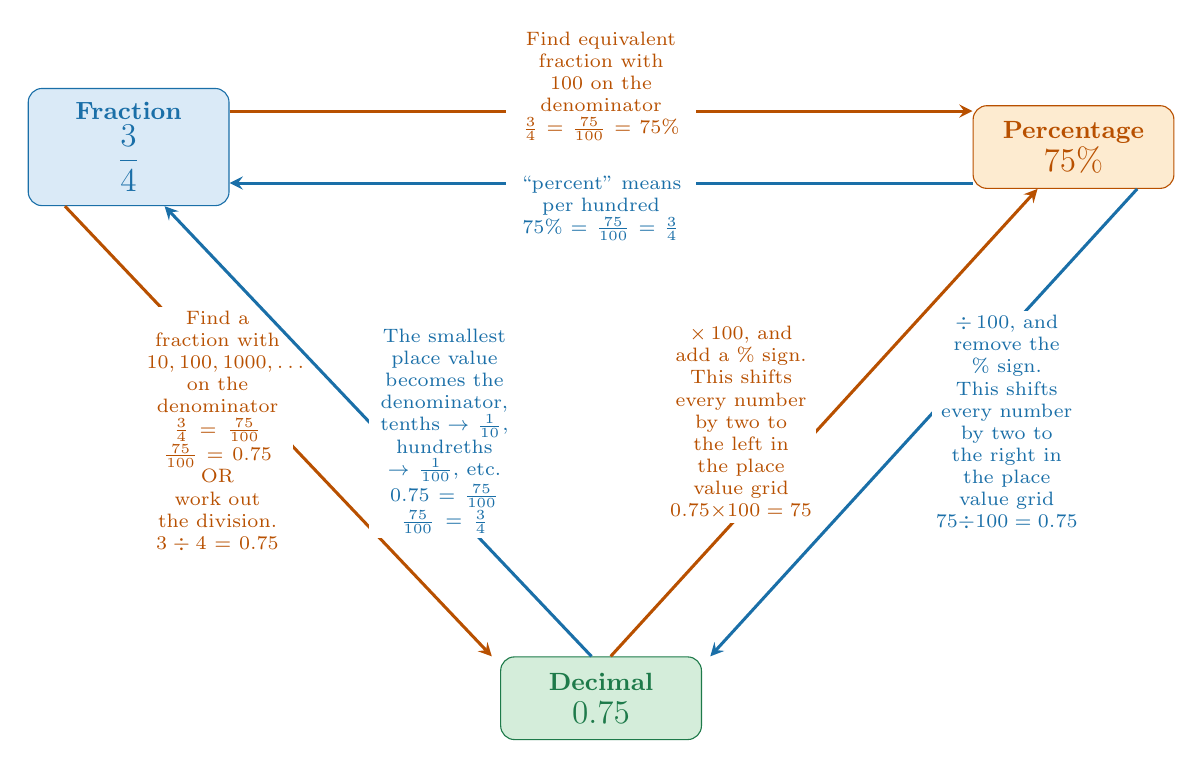
\begin{tikzpicture}[
  >=stealth,
  fwdarr/.style={->, line width=1.1pt, color=ArrowFwd},
  bckarr/.style={->, line width=1.1pt, color=ArrowBck},
  node/.style={font=\bfseries\small, inner sep=5pt, rounded corners=5pt,
               minimum width=2.55cm, minimum height=1.05cm, align=center},
  arrlbl/.style={font=\scriptsize, align=center, fill=white,
                 inner sep=1.5pt, text width=2.3cm},
  arrlblN/.style={font=\scriptsize, align=center, fill=white,
                  inner sep=1.5pt, text width=1.8cm},
]
  % Fraction: top-left
  \node[node, draw=MainBlue, fill=LightBlue, text=MainBlue]
    (F) at (0, 0)  {\bfseries Fraction\\[1pt]\large$\dfrac{3}{4}$};

  % Percentage: top-right
  \node[node, draw=AccentOrange, fill=LightOrange, text=AccentOrange]
    (P) at (12.0, 0) {\bfseries Percentage\\[1pt]\large$75\%$};

  % Decimal: bottom-centre
  \node[node, draw=AccentGreen, fill=LightGreen, text=AccentGreen]
    (D) at (6, -7) {\bfseries Decimal\\[1pt]\large$0.75$};

  %% F ↔ P  (top edge, above & below)
  \draw[fwdarr] ([yshift=13pt]F.east) -- ([yshift=13pt]P.west)
    node[midway, arrlbl, yshift=9pt]
      {\color{ArrowFwd} Find equivalent fraction with $100$ on the denominator $\frac{3}{4}=\frac{75}{100}=75\%$};
  \draw[bckarr] ([yshift=-13pt]P.west) -- ([yshift=-13pt]F.east)
    node[midway, arrlbl, yshift=-9pt]
      {\color{ArrowBck}``percent" means per hundred \\ $75 \% = \frac{75}{100}=\frac{3}{4}$};

  %% F ↔ D  (left edge)
  \draw[fwdarr] ([xshift=-23pt]F.south) -- ([xshift=-3pt]D.north west)
    node[midway, arrlblN, xshift=-22pt]
      {\color{ArrowFwd} Find a fraction with $10,100,1000,\dots$ on the denominator $\frac{3}{4}=\frac{75}{100}$ $ \frac{75}{100}=0.75$\\OR\\ work out the division.
      $3 \div 4 = 0.75$};
      
  \draw[bckarr] ([xshift= 33pt]D.north west) -- ([xshift= 13pt]F.south)
    node[midway, arrlblN, xshift=24pt]
      {\color{ArrowBck}The smallest place value becomes the denominator, tenths $\to \frac{1}{10}$, hundreths $\to \frac{1}{100}$, etc. \\
      $0.75=\frac{75}{100}$
      \\ $\frac{75}{100}=\frac{3}{4}$};

  %% D ↔ P  (right edge)
  \draw[fwdarr] ([xshift=-33pt]D.north east) -- ([xshift=-13pt]P.south)
    node[midway, arrlblN, xshift=-30pt]
      {\color{ArrowFwd}$\times\,100$, and add a \% sign. \\ This shifts every number by two to the left in the place value grid \\ $0.75\times100 = 75$};
  \draw[bckarr] ([xshift= 23pt]P.south) -- ([xshift= 3pt]D.north east)
    node[midway, arrlblN, xshift=30pt]
      {\color{ArrowBck}$\div\,100$, and remove the \% sign. \\ This shifts every number by two to the right in the place value grid \\ $75\div100=0.75$};

\end{tikzpicture}
\end{center}
\hfill

%% ══════════════════════════════════════════════════════════════════════════════
%% PLACE VALUE CHART (extended to ten‑thousands and ten‑thousandths)
\noindent\colorbox{PlaceHdr}{\makebox[\linewidth][l]{%
  \hspace{4pt}\color{white}\bfseries\footnotesize
  Place Value%
  \hspace{4pt}}}

\vspace{3pt}

\noindent
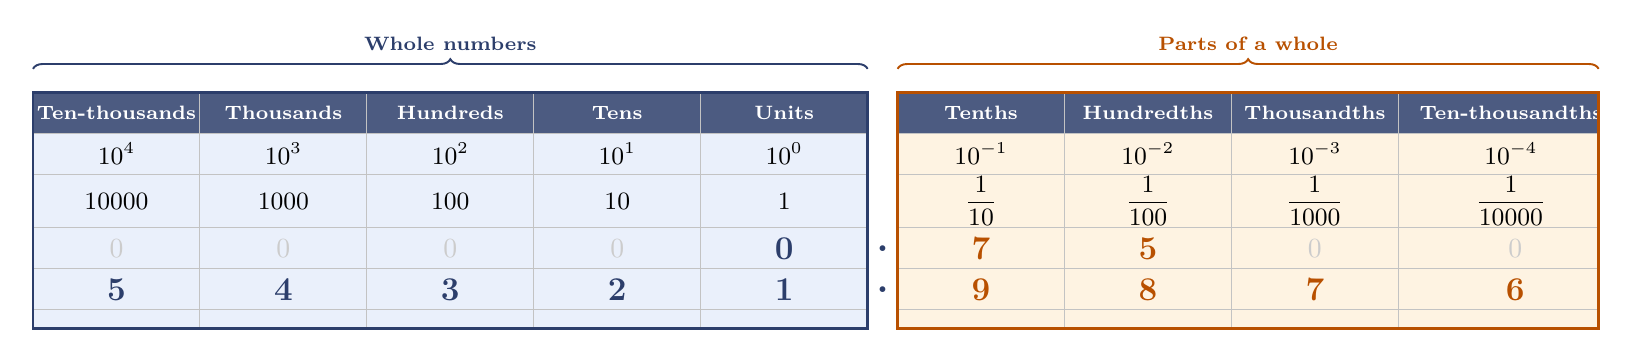
\begin{tikzpicture}[x=1cm, y=1cm]

  %% Column settings: 5 whole columns, dot column, 4 decimal columns
  \def\W{2.12}     % data column width
  \def\Wd{0.38}   % dot column width

  % Whole number column centres (x)
  \pgfmathsetmacro\cTenTho{\W*0.5}   % ten-thousands
  \pgfmathsetmacro\cTho{\W*1.5}     % thousands
  \pgfmathsetmacro\cHun{\W*2.5}     % hundreds
  \pgfmathsetmacro\cTen{\W*3.5}     % tens
  \pgfmathsetmacro\cUni{\W*4.5}     % units

  % Dot column
  \pgfmathsetmacro\xDot{\W*5}
  \pgfmathsetmacro\cDot{\W*5+\Wd*0.5}
  \pgfmathsetmacro\xDecStart{\W*5+\Wd}   % start of decimal columns

  % Decimal column centres
  \pgfmathsetmacro\cTth{\xDecStart+\W*0.5}      % tenths
  \pgfmathsetmacro\cHth{\xDecStart+\W*1.5}      % hundredths
  \pgfmathsetmacro\cTtth{\xDecStart+\W*2.5}     % thousandths
  \pgfmathsetmacro\cTenTth{\xDecStart+\W*3.7}   % ten-thousandths

  \pgfmathsetmacro\xRight{\xDecStart+\W*4.2}      % right border

  % Row y-coordinates (top of each row, counting down)
  \def\yTop{0}        % braces
  \def\yG{-0.3}       % top of grid
  \def\yHdr{-0.82}    % bottom of header row
  \def\yPow{-1.34}    % bottom of powers row
  \def\yVal{-2.02}    % bottom of values row (taller for fractions)
  \def\yEx{-2.54}     % bottom of example row 1
  \def\yExB{-3.06}    % bottom of example row 2
  \def\yBot{-3.3}     % bottom of grid

  %% Background fills
  \fill[PlaceWhole] (0,\yG) rectangle (\W*5, \yBot);
  \fill[PlaceDec]   (\xDecStart,\yG) rectangle (\xRight, \yBot);
  \fill[PlaceHdr!85] (0,\yG) rectangle (\W*5, \yHdr);
  \fill[PlaceHdr!85] (\xDecStart,\yG) rectangle (\xRight, \yHdr);
  \fill[white] (\xDot,\yG) rectangle (\xDecStart,\yBot);

  %% Braces above (whole vs decimal)
  \draw[decorate, decoration={brace,amplitude=3.5pt}, PlaceHdr, line width=0.7pt]
    (0,\yTop) -- (\W*5,\yTop)
    node[midway, above=3pt, font=\bfseries\scriptsize, text=PlaceHdr]
      {Whole numbers};
  \draw[decorate, decoration={brace,amplitude=3.5pt}, AccentOrange, line width=0.7pt]
    (\xDecStart,\yTop) -- (\xRight,\yTop)
    node[midway, above=3pt, font=\bfseries\scriptsize, text=AccentOrange]
      {Parts of a whole};

  %% Header row labels
  \foreach \cx/\lbl in {
    \cTenTho/Ten-thousands, \cTho/Thousands, \cHun/Hundreds,
    \cTen/Tens, \cUni/Units,
    \cTth/Tenths, \cHth/Hundredths, \cTtth/Thousandths, \cTenTth/Ten-thousandths
  }{
    \node[font=\bfseries\scriptsize, text=white, align=center]
      at (\cx, {(\yG+\yHdr)/2}) {\lbl};
  }

  %% Powers of 10 row
  \foreach \cx/\pw in {
    \cTenTho/$10^{4}$, \cTho/$10^{3}$, \cHun/$10^{2}$, \cTen/$10^{1}$, \cUni/$10^{0}$,
    \cTth/$10^{-1}$, \cHth/$10^{-2}$, \cTtth/$10^{-3}$, \cTenTth/$10^{-4}$
  }{
    \node[font=\small, align=center] at (\cx, {(\yHdr+\yPow)/2}) {\pw};
  }

  %% Values row
  \foreach \cx/\vl in {
    \cTenTho/{$10000$},
    \cTho/{$1000$},
    \cHun/{$100$},
    \cTen/{$10$},
    \cUni/{$1$},
    \cTth/{$\dfrac{1}{10}$},
    \cHth/{$\dfrac{1}{100}$},
    \cTtth/{$\dfrac{1}{1000}$},
    \cTenTth/{$\dfrac{1}{10000}$}
  }{
    \node[align=center, font=\small] at (\cx, {(\yPow+\yVal)/2}) {\vl};
  }

  %% Example 1: 0.75 (uses units, tenths, hundredths)
  \foreach \cx/\dg in {
    \cTenTho/{\color{gray!40}0},
    \cTho/{\color{gray!40}0},
    \cHun/{\color{gray!40}0},
    \cTen/{\color{gray!40}0},
    \cUni/{\large\bfseries\color{PlaceHdr}0},
    \cTth/{\large\bfseries\color{AccentOrange}7},
    \cHth/{\large\bfseries\color{AccentOrange}5},
    \cTtth/{\color{gray!40}0},
    \cTenTth/{\color{gray!40}0}
  }{
    \node at (\cx, {(\yVal+\yEx)/2}) {\dg};
  }
  % \node[font=\small\bfseries, text=AccentOrange] at (\xRight+0.55, {(\yVal+\yEx)/2})
  %   {$= 0.75$};

  %% Example 2: 54321.9876 (demonstrates ten‑thousands and ten‑thousandths)
  \foreach \cx/\dg in {
    \cTenTho/{\large\bfseries\color{PlaceHdr}5},
    \cTho/{\large\bfseries\color{PlaceHdr}4},
    \cHun/{\large\bfseries\color{PlaceHdr}3},
    \cTen/{\large\bfseries\color{PlaceHdr}2},
    \cUni/{\large\bfseries\color{PlaceHdr}1},
    \cTth/{\large\bfseries\color{AccentOrange}9},
    \cHth/{\large\bfseries\color{AccentOrange}8},
    \cTtth/{\large\bfseries\color{AccentOrange}7},
    \cTenTth/{\large\bfseries\color{AccentOrange}6}
  }{
    \node at (\cx, {(\yEx+\yExB)/2}) {\dg};
  }
  % \node[font=\small\bfseries, text=AccentGreen] at (\xRight+1.0, {(\yEx+\yExB)/2})
  %   {$= 54321.9876$};

  %% Decimal points
  \node[font=\Large\bfseries, text=PlaceHdr] at (\cDot, {(\yVal+\yEx)/2})  {.};
  \node[font=\Large\bfseries, text=PlaceHdr] at (\cDot, {(\yEx+\yExB)/2}) {.};

  %% Grid lines
  \foreach \y in {\yG, \yHdr, \yPow, \yVal, \yEx, \yExB, \yBot}{
    \draw[DotCol!50, line width=0.35pt] (0,\y) -- (\W*5,\y);
    \draw[DotCol!50, line width=0.35pt] (\xDecStart,\y) -- (\xRight,\y);
  }
  \foreach \x in {0, \W, \W*2, \W*3, \W*4, \W*5}{
    \draw[DotCol!50, line width=0.35pt] (\x,\yG) -- (\x,\yBot);
  }
  \foreach \x in {\xDecStart, \xDecStart+\W, \xDecStart+\W*2, \xDecStart+\W*3, \xRight}{
    \draw[DotCol!50, line width=0.35pt] (\x,\yG) -- (\x,\yBot);
  }

  %% Outer borders
  \draw[PlaceHdr, line width=0.9pt] (0,\yG) rectangle (\W*5, \yBot);
  \draw[AccentOrange, line width=0.9pt] (\xDecStart,\yG) rectangle (\xRight, \yBot);

\end{tikzpicture}

%% ══════════════════════════════════════════════════════════════════════════════
%% EXTENDED EQUIVALENTS TABLE (left) + THREE CONVERSION TRIANGLES (right)
\vspace{1pt}
\noindent
\begin{minipage}[t]{0.18\linewidth}
\vspace{0pt}
\noindent\colorbox{TitleBg}{\makebox[\linewidth][l]{%
  \hspace{3pt}\color{white}\bfseries\scriptsize Key Conversions \hspace{3pt}}}
\par\vspace{2pt}
\renewcommand{\arraystretch}{2.0}
{\scriptsize\setlength{\tabcolsep}{2pt}
\rowcolors{2}{RowAlt}{white}
\begin{tabular}{
  >{\bfseries\centering\arraybackslash}p{1.1cm}
  >{\bfseries\centering\arraybackslash}p{1.1cm}
  >{\bfseries\centering\arraybackslash}p{1.1cm}
}
\rowcolor{RowAlt}
Fraction & Decimal & \% \\
$100$  & $100$       & $10,000\%$         \\
$10$  & $10$       & $1000\%$         \\
$1$  & $1$       & $100\%$         \\
$\tfrac{1}{10}$  & $0.1$      & $10\%$         \\
$\tfrac{1}{100}$  & $0.01$      & $1\%$         \\
$\tfrac{1}{1000}$  & $0.001$       & $0.1\%$         \\
$\tfrac{1}{10,000}$  & $0.0001$       & $0.01\%$         \\
$\tfrac{1}{2}$  & $0.5$       & $50\%$         \\
$\tfrac{1}{3}$  & $0.\dot{3}$       & $33.\dot{3}\%$         \\
$\tfrac{2}{3}$  & $0.\dot{6}$       & $66.\dot{6}\%$         \\
$\tfrac{1}{4}$  & $0.25$       & $25\%$         \\
$\tfrac{3}{4}$  & $0.75$     & $75\%$       \\
$\tfrac{1}{5}$  & $0.2$     & $20\%$       \\
$\tfrac{1}{6}$  & $0.1\dot{6}$     & $16.\dot{6}\%$       \\
$\tfrac{1}{7}$  & $0.\dot{1}4285\dot{7}$     & $14.28...\%$       \\
$\tfrac{1}{8}$  & $0.125$ & $12.5\%$ \\
$\tfrac{1}{9}$  & $0.\dot{1}$ & $11.\dot{1}\%$ \\
$\tfrac{1}{20}$  & $0.05$ & $5\%$ \\
$\tfrac{1}{25}$  & $0.04$ & $4\%$ \\
$\tfrac{1}{50}$  & $0.02$ & $2\%$ \\
\end{tabular}
}
\end{minipage}\hfill
\begin{minipage}[t]{0.80\linewidth}
\vspace{0pt}
\centering
\colorbox{TitleBg}{\makebox[\linewidth][l]{%
  \hspace{3pt}\color{white}\bfseries\scriptsize More Examples\hspace{3pt}}}
\par\vspace{3pt}
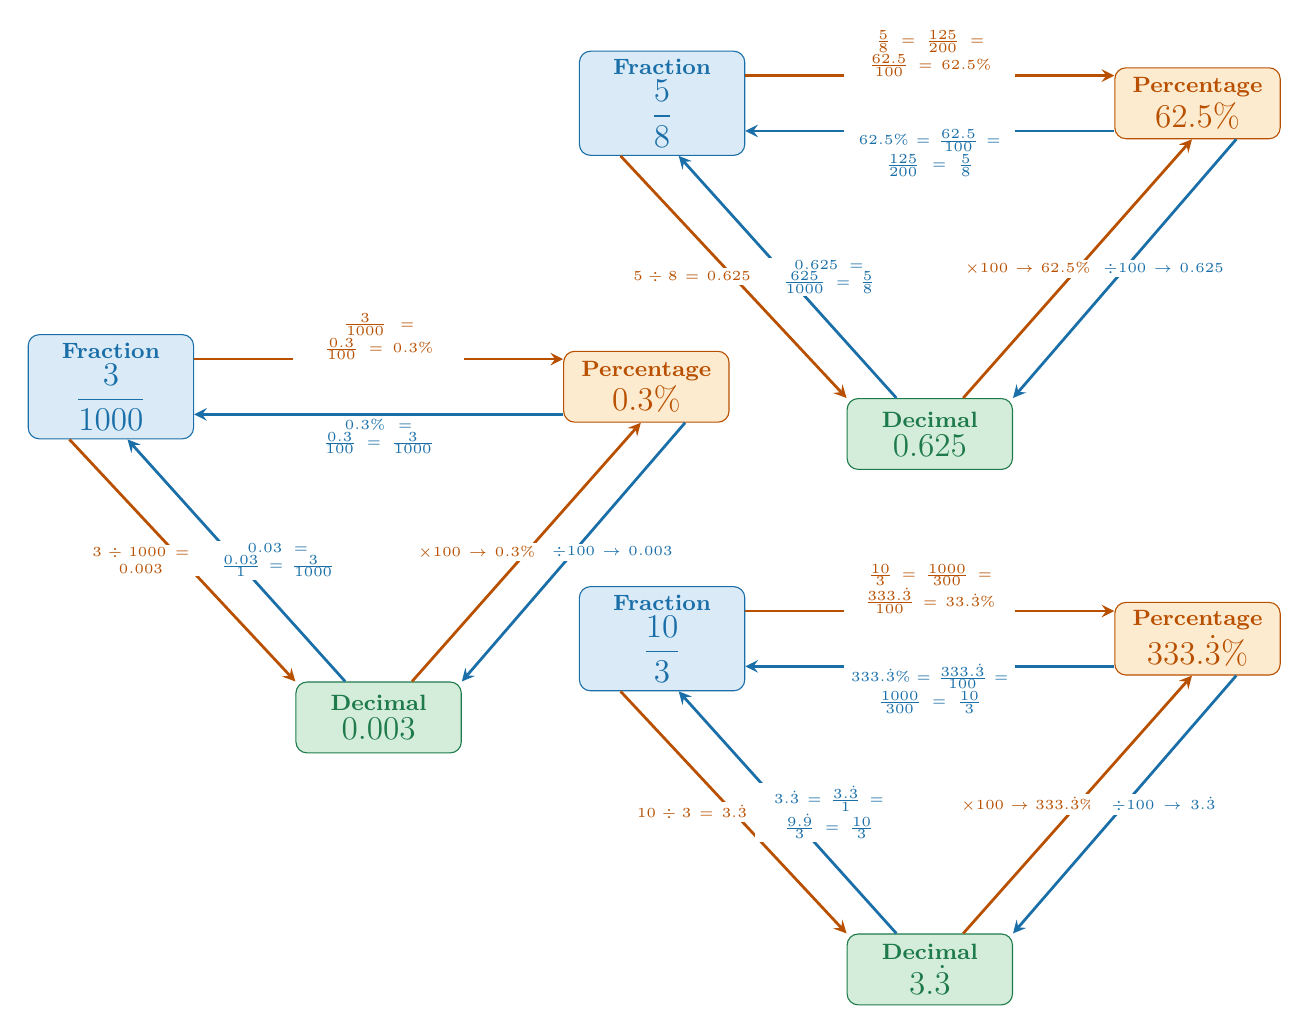
\begin{tikzpicture}[
  >=stealth,
  fwdarr/.style={->, line width=1pt, color=ArrowFwd},
  bckarr/.style={->, line width=1pt, color=ArrowBck},
  node/.style={font=\bfseries\footnotesize, inner sep=3pt, rounded corners=4pt,
               minimum width=2.1cm, minimum height=0.9cm, align=center},
  arrlbl/.style={font=\tiny, align=center, fill=white, inner sep=1pt, text width=2.1cm},
  arrlblN/.style={font=\tiny, align=center, fill=white, inner sep=1pt, text width=1.8cm},
]

% ===== Triangle 1 (top) : 5/8 = 0.625 = 62.5% =====
  \node[node, draw=MainBlue, fill=LightBlue, text=MainBlue]
    (F1) at (5,0) {\bfseries Fraction\\[1pt]\large$\dfrac{5}{8}$};
  \node[node, draw=AccentOrange, fill=LightOrange, text=AccentOrange]
    (P1) at (11.8,0) {\bfseries Percentage\\[1pt]\large$62.5\%$};
  \node[node, draw=AccentGreen, fill=LightGreen, text=AccentGreen]
    (D1) at (8.4,-4.2) {\bfseries Decimal\\[1pt]\large$0.625$};
  \draw[fwdarr] ([yshift=10pt]F1.east) -- ([yshift=10pt]P1.west)
    node[midway, arrlbl, yshift=8pt] {\color{ArrowFwd} $\frac{5}{8}=\frac{125}{200}=\frac{62.5}{100}=62.5\%$};
  \draw[bckarr] ([yshift=-10pt]P1.west) -- ([yshift=-10pt]F1.east)
    node[midway, arrlbl, yshift=-8pt] {\color{ArrowBck} $62.5\% = \frac{62.5}{100}=\frac{125}{200}=\frac{5}{8}$};
  \draw[fwdarr] ([xshift=-15pt]F1.south) -- ([xshift=0pt]D1.north west)
    node[midway, arrlblN, xshift=-15pt] {\color{ArrowFwd} $5\div8 = 0.625$};
  \draw[bckarr] ([xshift=18pt]D1.north west) -- ([xshift=6pt]F1.south)
    node[midway, arrlblN, xshift=15pt] {\color{ArrowBck} $0.625=\frac{625}{1000}=\frac{5}{8}$};
  \draw[fwdarr] ([xshift=-18pt]D1.north east) -- ([xshift=-2pt]P1.south)
    node[midway, arrlblN, xshift=-18pt] {\color{ArrowFwd} $\times100 \to 62.5\%$};
  \draw[bckarr] ([xshift=14pt]P1.south) -- ([xshift=0pt]D1.north east)
    node[midway, arrlblN, xshift=14pt] {\color{ArrowBck} $\div100 \to 0.625$};

% ===== Triangle 2 (middle, offset left) : 10/3 = 3.333... = 333.33...% =====
  \node[node, draw=MainBlue, fill=LightBlue, text=MainBlue]
    (F2) at (5.0,-6.8) {\bfseries Fraction\\[1pt]\large$\dfrac{10}{3}$};
  \node[node, draw=AccentOrange, fill=LightOrange, text=AccentOrange]
    (P2) at (11.8,-6.8) {\bfseries Percentage\\[1pt]\large$333.\dot{3}\%$};
  \node[node, draw=AccentGreen, fill=LightGreen, text=AccentGreen]
    (D2) at (8.4,-11.0) {\bfseries Decimal\\[1pt]\large$3.\dot{3}$};
  \draw[fwdarr] ([yshift=10pt]F2.east) -- ([yshift=10pt]P2.west)
    node[midway, arrlbl, yshift=8pt] {\color{ArrowFwd} $\frac{10}{3}=\frac{1000}{300}=\frac{333.\dot{3}}{100}=33.\dot{3}\%$};
  \draw[bckarr] ([yshift=-10pt]P2.west) -- ([yshift=-10pt]F2.east)
    node[midway, arrlbl, yshift=-8pt] {\color{ArrowBck} $333.\dot{3}\% = \frac{333.\dot{3}}{100}=\frac{1000}{300}=\frac{10}{3}$};
  \draw[fwdarr] ([xshift=-15pt]F2.south) -- ([xshift=0pt]D2.north west)
    node[midway, arrlblN, xshift=-15pt] {\color{ArrowFwd} $10\div3 = 3.\dot{3}$};
  \draw[bckarr] ([xshift=18pt]D2.north west) -- ([xshift=6pt]F2.south)
    node[midway, arrlblN, xshift=15pt] {\color{ArrowBck} $3.\dot{3}=\frac{3.\dot{3}}{1}=\frac{9.\dot{9}}{3}=\frac{10}{3}$};
  \draw[fwdarr] ([xshift=-18pt]D2.north east) -- ([xshift=-2pt]P2.south)
    node[midway, arrlblN, xshift=-18pt] {\color{ArrowFwd} $\times100 \to 333.\dot{3}\%$};
  \draw[bckarr] ([xshift=14pt]P2.south) -- ([xshift=0pt]D2.north east)
    node[midway, arrlblN, xshift=14pt] {\color{ArrowBck} $\div100 \to 3.\dot{3}$};

% ===== Triangle 3 (bottom) : 3/1000 = 0.003 = 0.3% =====
  \node[node, draw=MainBlue, fill=LightBlue, text=MainBlue]
    (F3) at (-2,-3.6) {\bfseries Fraction\\[1pt]\large$\dfrac{3}{1000}$};
  \node[node, draw=AccentOrange, fill=LightOrange, text=AccentOrange]
    (P3) at (4.8,-3.6) {\bfseries Percentage\\[1pt]\large$0.3\%$};
  \node[node, draw=AccentGreen, fill=LightGreen, text=AccentGreen]
    (D3) at (1.4,-7.8) {\bfseries Decimal\\[1pt]\large$0.003$};
  \draw[fwdarr] ([yshift=10pt]F3.east) -- ([yshift=10pt]P3.west)
    node[midway, arrlbl, yshift=8pt] {\color{ArrowFwd} $\frac{3}{1000}=\frac{0.3}{100}=0.3\%$};
  \draw[bckarr] ([yshift=-10pt]P3.west) -- ([yshift=-10pt]F3.east)
    node[midway, arrlbl, yshift=-8pt] {\color{ArrowBck} $0.3\% = \frac{0.3}{100}=\frac{3}{1000}$};
  \draw[fwdarr] ([xshift=-15pt]F3.south) -- ([xshift=0pt]D3.north west)
    node[midway, arrlblN, xshift=-15pt] {\color{ArrowFwd} $3\div1000 =$\\$ 0.003$};
  \draw[bckarr] ([xshift=18pt]D3.north west) -- ([xshift=6pt]F3.south)
    node[midway, arrlblN, xshift=15pt] {\color{ArrowBck} $0.03=\frac{0.03}{1}=\frac{3}{1000}$};
  \draw[fwdarr] ([xshift=-18pt]D3.north east) -- ([xshift=-2pt]P3.south)
    node[midway, arrlblN, xshift=-18pt] {\color{ArrowFwd} $\times100 \to 0.3\%$};
  \draw[bckarr] ([xshift=14pt]P3.south) -- ([xshift=0pt]D3.north east)
    node[midway, arrlblN, xshift=14pt] {\color{ArrowBck} $\div100 \to 0.003$};

\end{tikzpicture}
\end{minipage}

\vspace{6pt}
\end{document}